% ==================================================================================================================================
% Définitions et propriétés

\minitoc  % Affiche la table des matières pour ce chapitre

Les équations différentielles font partie intégrante de la vie de tous les jours. 
En effet, elles permettent de modéliser des phénomènes qui varient dans le temps. 
Du plus simple comme le reffroidissement d'une tasse de café, au plus complexe tels que la modélisation 
de phénomène quantiques ou climatilogiques. 

Nous allons ici définir formellement les équations différentielles. Nous nous attarderons ensuite sur 
les deux grands types d'équations : les équations différentielles linéaires et non linéaires. 
Nous finirons par une introduction à l'étude qualitative. 

% ==================================================================================================================================
% Équations différentielles - généralités

\section{Équations différentielles - généralités}

Nous allons chercher dans ce cours à définir proprement la notion d'équation différentielles, 
de solution d'une équation différentielle et voir quelques propriétés de ces deux objets. 

\subsection{Définitions et premières propriétés}

\begin{definition}[Equation Différentielle Scalaire]
    Soit $f : \Omega \longrightarrow \K$ où $ \Omega \subseteq \R \times \K^N$ avec $N \in \N$. 
    L'équation différentielle associée à $f$ est :
        \[ (E) : y^{(n)} = f(t,y,\dots,y^{(n-1)}) \] 
    On appelle cela une \textbf{équation différentielle d'ordre n scalaire}. 
    On peut appeler $f$ la fonction décrivant l'équation différentielle. 
\end{definition}

Définissons maintenant clairement le concept de "solution" d'une équation différentielle. 

\begin{definition}[Solution]
    Une fonction $y$ est appelée solution d'une équation différentielle $(E)$ d'ordre $n \in \N$ 
    définie par la fonction $f$ si :
    \begin{itemize}
        \item $y : I \longrightarrow \K$ est $n$ fois dérivable 
        \item $ \forall t \in I, \quad (t,y(t), \dots, y^{(n-1)}(t)) \in \Omega $ 
        \item $ \forall t \in I$, on a : 
            \[ \boxed{ y^{(n)}(t) = f(t,y(t), \dots, y^{(n-1)}(t)) } \] 
    \end{itemize}
\end{definition}

\begin{remark}
    Si on change l'intervalle de définition $I$ d'une solution d'une équation différentielle, 
    alors on change aussi la solution. Autrement dit, une solution est très dépendante de son intervalle 
    de définition. On peut donc parfois noter $(I,y)$ une solution $y$ définie sur un intervalle $I$. 
\end{remark}

\begin{definition}[Equation Différentielle Vectorielle]
    Soit $f : \Omega \longrightarrow \K^N$ avec $n \in \N^*$ et $\Omega \subseteq \R \times (\K^N)^N$. 
    L'équation différentielle ordinaire associée à $f$ est :
        \[ (E) : y^{(n)} = f(t,y,\dots,y^{(n-1)}) \] 
    On peut écrire cette équation différentielle sous forme de système d'équations différentielles 
    en décomposant les différentes composantes de l'équation différentielle tel que :
        \[
            \begin{cases}
                y_1^{(n)} = f_1(t,y_1, \dots, y_N^{(n-1)}) \\ 
                \vdots \quad  \quad \quad \quad \quad \quad \quad \vdots \\ 
                y_N^{(n)} = f_1(t,y_N, \dots, y_N^{(n-1)}) \\ 
            \end{cases} 
        \]
\end{definition}

Lors de l'étude d'un equation différentielle d'ordre $n$, un théorème que nous verrons plus tard nous permettra
de nous ramener à l'étude d'une équation différentielle d'ordre $1$. 
Il est donc important de bien comprendre ce qu'est une équation différentielle d'ordre $1$. 

\begin{remark}[Equation Differentielle d'ordre 1]
    Soit $f : \Omega \longrightarrow \K^N $ où $ \Omega \subseteq \R \times \K^N$. 
    L'équation différentielle associée à $f$ est :
        \[ (E) : y' = f(t,y) \] 
\end{remark}

\begin{example}
    Voyons quelques exemples d'équations différentielles : 
    \begin{itemize}
        \item $\K = \R, N = 1, n = 1, \Omega = \R \times \R$ et $f(t,x) = x $ 
            \[ (E) : y' = y \] 
        \item $\K = \R, N = 2, n = 1, \Omega = \R \times \R^2$
            \[ f : 
                \begin{cases}
                    \Omega \longrightarrow \R^2 \\ 
                    (t,x) \longmapsto Ax + B 
                \end{cases}
                \text{ où } B \in \R^2 \text{ et } A \in \mathcal{M}_2(\R) \] 
            \[ (E) : y' = Ay + B \] 
            \[ (E) : 
                \begin{cases}
                    y_1' = a_{1,1}y_1 + a_{1,2}y_2 + b_1 \\ 
                    y_2' = a_{2,1}y_1 + a_{2,2}y_2 = b_2
                \end{cases}
            \]
        \item $\K = \C, N = 1, n = 1, \Omega = \R \times \C$ 
            \[ f : 
                \begin{cases}
                    \Omega \longrightarrow \C \\ 
                    (t,z) \longmapsto z^2 + t 
                \end{cases}
                \quad \text{ et } \quad 
                (E) : y' = y^2 + t 
            \]
    \end{itemize}
\end{example}

Lors de la résolution d'une équation différentielle, on remarque que on trouve la plupart du temps une infinité de 
solutions. Parfois, une unique solution serait plus pratique (ex : en physique). On va donc chercher à donner des 
conditions supplémentaires sur la fonction solution en imposant une de ses valeurs. 

\begin{definition}[Problème de Cauchy]
    Soit $(E)$ une équation différentielle ordinaire d'ordre 1, de fonction descriptive $f$ et de la forme $y' = f(t,x)$. 
    Résoudre un problème de Cauchy associé à $(E)$ consiste à trouver une solution de $(E)$ qui vérifie un condition initiale : 
    \[ (C) : y(t_0) = y_0 \quad \text{ où } (t_0,y_0) \in \Omega \] 
\end{definition}

\begin{proposition}[Exercice]
    Soit $f : \Omega \subset \R \times \K^N \longrightarrow \K^N$ et $(E)$ l'équation associée d'ordre 1 :
        \[ y' = f(t,y) \] 
    Alors : $y : I \longrightarrow \K^N$ est solution du problème de Cauchy :
        \[ (P) : 
            \begin{cases}
                (E) : y' = f(t,y) \\ 
                (C) : y(t_0) = y_0 
            \end{cases}
        \] 
    si et seulement si 
        \begin{itemize}
            \item $y \in \mathcal{C}^0(I)$ 
            \item $ \forall t \in I, \quad (t,y(t)) \in \Omega $ 
            \item $ \forall t \in I$, 
                \[ y(t) = y_0 + \int_{t_0}^{t} f(s,y(s)) \; ds \] 
        \end{itemize}
\end{proposition}

\begin{definition}[Solution Maximale]
    $y$ est une solution maximale de $(E)$ si il n'existe pas de prolongement strict de $y$ en une solution de $(E)$. 
\end{definition}

\begin{definition}[Solution Globale]
    Soit $(E) : y' = f(t,y)$ où $f : I \times \Omega \longrightarrow \K^N$. 
    On dit que $y$ est une solution globale de $(E)$ si $y$ est une solution de $(E)$ et qu'elle est définie sur $I$.
\end{definition}

\begin{remark}
    Une solution globale est maximale. La réciproque est fausse, voyons un exemple. 
        \[ (E) : y' = y^2 \quad \text{ et } \quad y_s :
            \begin{cases}
                A \longrightarrow \R \\ 
                t \longmapsto - \frac{1}{t}
            \end{cases}
            \text{où } f: 
            \begin{cases}
                \R \times \R \longrightarrow \R \\ 
                (t,x) \longmapsto x^2
            \end{cases}
            \quad \text{ et } \quad A = \R_+^* \] 
    $y_s$ n'est pas une solution globale car on ne peut pas la prolonger en une fonction continue solution de $(E)$. 
    En revanche, c'est une solution maximale. 
\end{remark}

\begin{theorem}[Existence et Unicité de solution maximale]
    Il existe une solution maximale d'un problème de Cauchy. 
\end{theorem}


\subsection{Première méthode résolution}

A partir des outils que nous avons à notre porté, nous pouvons dès à présent déterminer la forme de l'ensemble des solution 
d'une équation différentielle scalaire homogène d'ordre 1. Soient $I$ un intervalle, $a : I \longrightarrow \K$ une fonction continue 
et $(E)$ une équation différentielle de la forme : 
    \[ (E) : y' = a(t)y = f(t,y) \quad \text{où} \quad f : 
        \begin{cases}
            I \times \K \longrightarrow \K \\ 
            (t,x) \longmapsto a(t)x
        \end{cases}
    \]
Soit le problème de Cauchy suivant : 
    \[ (P) : 
        \begin{cases}
            (E) : y' = a(t)y = f(t,y) \\ 
            y(t_0) = y_0
        \end{cases}
        \quad \text{où} \quad (t_0,y_0) \in I \times \K \] 
On cherche la forme générale de l'ensemble des solutions du problème de Cauchy. 

\subsubsection{Existence d'une solution}

Soit $y : I \longrightarrow \K, t \longmapsto e^{ \int_{t_0}^{t} a}$. Montrons que $y$ est bien une solution maximale du 
problème de Cauchy. 
\begin{itemize}
    \item Soit $t \in I$ alors $y(t) \in \K$ 
    \item $ \forall t \in I$, on a : $y'(t) = y_0 a(t) e^{ \int_{t_0}^{t} a}$ 
    Donc $y$ est bien une solution de $(E)$. De plus, $y$ est une solution globale donc elle est maximale. 
    \item Condition initiale : 
        \[ y(t_0) = y_0 e^{ \int_{t_0}^{t_0} a} = y_0 e^0 = y_0 \] 
    On a donc que $y$ est bien une solution maximale du problème de Cauchy énoncé. 
\end{itemize}

\subsubsection{Unicité de la solution}

Soit $u : J \subset I \longrightarrow \K$ une solution maximale de $(E)$ telle que $t_0 \in J$ et $u(t_0) = y_0$. 

Montrons que la fonction $v : t \longmapsto u(t) e^{ - \int_{t_0}^{t} a}$ est constante. 
$v$ est dérivable par composition/produit. On a donc $ \forall t \in J$, 
    \begin{align*}
        y'(t) &= u'(t) \times e^{ \int_{t_0}^{t} a} - u(t)a(t)e^{ \int_{t_0}^{t} a} \\ 
              &= e^{ \int_{t_0}^{t} a} (u'(t) - u(t)a(t))
    \end{align*}
or $u$ est un solution maximale de $(E)$ donc $ \forall t \in J, u'(t) = a(t)u(t) \iff u'(t) - u(t)a(t) = 0$ d'où :
    \[ y'(t) = 0 \] 
Donc $v$ est une fonction constante sur $J$. Déterminons cette constante. 
    \[ v(t_0) = u(t_0) e^{ - \int_{t_0}^{t_0} a} = u(t_0)e^0 = u(t_0) = y_0 \] 
Donc $ \forall t \in J, \; v(t) = y_0 $. 

Montrons que $u = y_{ |J}$ et que $I = J$. Soit $t \in J$, on a :
    \begin{align*}
        & v(t) = u(t) e^{ - \int_{t_0}^{t_0} a} \\ 
        \iff & u(t) = v(t) e^{ \int_{t_0}^{t_0} a} \\ 
        & u(t) = y_0 e^{ \int_{t_0}^{t_0} a} 
    \end{align*}
Donc $u = y_{ |J}$. De plus, $y$ est un prolongement de $u$ or $u$ est supposée maximale (i.e elle n'admet pas de prolongement solution)
donc $I = J$. 

\subsubsection{Conclusion}

Enfin, ces calculs nous permettent d'énoncer le résultat suivant : 

\begin{theorem}[Solutions d'une ED scalaire homogène d'ordre 1]
    Soient $I$ un intervalle, $a : I \longrightarrow \K$ une fonction continue et $f : I \times \K \longrightarrow \K$. 

    Soit $(E) : y' = a(t)y = f(t,y)$ l'équation différentielle homogène d'ordre 1 associée à $f$. 
    Soient $(t_0, y_0) \in I \times \K$, et $(P) : \{(E), y(t_0) = y_0\}$ un problème de Cauchy. 
    Alors les solutions maximales de $(P)$ sont exactement les fonctions de la forme : 
        \[ y : 
            \begin{cases}
                I \longrightarrow \K \\ 
                t \longmapsto y_0 \exp \left( \int_{t_0}^{t} a(s) \; ds \right)
            \end{cases}
        \] 
\end{theorem}

% ==================================================================================================================================
% Équations différentielles Linéaires

\section{Équations différentielles Linéaires}


\subsection{Notions d'analyse Matricielle}

Soient $E$ et $F$ deux espaces vectoriels normés. $ \mathcal{L}(E,F)$ désigne l'espace vectoriel des applications linéaires 
de E vers F. Il est muni d'une norme appelée \textbf{norme opérationnelle} : 
    \[ \forall f \in \mathcal{L}(E,F), \quad \| f \| = \min \{ C \in \R_+ \; | \; \forall x \in E, \| f(x) \|_F \leqslant C \| x \|_E \} \]

\begin{definition}[Norme Subordonnée]
    Si $\|.\|$ est une norme sur $\K^n$ alors la norme subordonnée associée à $\|.\|$ sur $ \mathcal{M}_n(\K)$ est 
    la norme opérationnelle associée à $\|.\|$ sur $\K^n = E$ et $\|.\|$ sur $\K^n = F$. On la note de la même façon. 
    \[ \text{i.e} \quad \forall M \in \mathcal{M}_n(\K), \quad  \| M \| = \min \{ C \in \R_+ \; | \; \forall x \in \K^n, \| Mx \| \leqslant C \| x \| \} \]
\end{definition}

\begin{proposition}
    Soient $M,N \in \mathcal{M}_n(\K)$ alors :
        \[ \| M \times N \| \leqslant \|M\| \times \|N\| \]
    Ceci d'écoule de l'inégalité de Cauchy-Schwarz. 
\end{proposition}

\begin{remark}
    Soit $f : I \longrightarrow \mathcal{M}_n(\K)$ où I est un intervalle. Supposons que $f$ soit continue. 
    On peut alors définir $ \int_I f(t) \; dt \in \mathcal{M}_n(\K)$ composante par composante telle que :
        \[ \left( \int_I f(t) \; dt \right)_{i,j} = \int_I f(t)_{i,j} \; dt \] 
    Autrement dit, l'intégrale d'une matrice d'applications continues sur un intervalle est exactement la matrice 
    les intégrales des applications. 
\end{remark}

\begin{proposition}
    Soit $f : I = ]a,b[ \overset{ \mathcal{C}^0}{\longrightarrow} \mathcal{M}_n(\K)$. Alors :
        \[ \left\| \int_I f(t) \; dt \right\| \leqslant \int_{a}^{b} \left\| f(t) \right\| \; dt \] 
\end{proposition}

\begin{prop}[Théorème Fondamental de l'Analyse]
    Dans ce cas ci, le théorème fondamental de l'analyse est toujours vrai. 
    Autrement dit, soit $f : I = ]a,b[ \overset{ \mathcal{C}^0}{\longrightarrow} \mathcal{M}_n(\K)$. 
    Alors : 
        \[ \int_{a}^{b} f'(t) \; dt = f(b) - f(a) \] 
\end{prop}

\begin{remark}
    Soit $f \in \mathcal{C}^1(I, \mathcal{M}_n(\K))$. Alors la formule $(f^2)' = 2f'f$ est fausse 
    puisque $\mathcal{M}_n(\K)$ n'est pas un anneau commutatif. D'où : 
        \[ (fg)' = f'g + fg' \quad \text{où} \quad g \in \mathcal{C}^1(I, \mathcal{M}_n(\K)) \] 
\end{remark}

\begin{remark}
    Pour rappel, on sait que $ \forall z \in \C, \; e^z = \sum_{k=0}^{\infty} \frac{z^k}{k!}$. 
\end{remark}

\begin{definition}[Exponentielle d'une matrice]
    Soit $A \in \mathcal{M}_n(\K)$ on a alors :
        \[ \exp(A) := \sum_{k=0}^{\infty} \frac{A^k}{k!} \]
    Cette série converge toujours. 
\end{definition}

\begin{proposition}[Propriétés de l'exponentielle]
    Soient $A,B \in \mathcal{M}_n(\K)$ alors 
        \[ e^{A+B} = e^A e^B \iff AB = BA \] 
\end{proposition}

\begin{proposition}[Inverse]
    Soit $A \in \mathcal{M}_n(\K)$ alors $e^A$ est inversible. 
    Pour cela, on pose :
    \[ e^0 = \sum_{k=0}^{\infty} \frac{O^k}{k!} = 1_{\mathcal{M}_n(\K)} = I_n \quad \text{et} \quad e^{(A+ (-A))} = e^A e^{-A} = I_n \] 
\end{proposition}

\begin{prop}[Dérivation de l'exponentielle matricielle] 
		\begin{itemize} 
			\item Soit $A \in \mathcal{A}_n(\K)$. La fonction:
			\[ 
				\begin{cases} 
					\R \longrightarrow \mathcal{M}_n(\K) \\ 
					t \longmapsto e^{tA} 
				\end{cases}
			\]
			est de classe $ \mathcal{C}^\infty$ sur $\R$ et: 
					\[ \boxed{ \frac{\partial e^{tA}}{\partial t} = A e^{tA} = e^{tA} A } \]
			\item Soit $A \in \mathcal{C}^1(\R, \mathcal{M}_n(\K))$ telle que 
			$ \forall t \in \R, A(t)A'(t) = A'(t) A(t)$  alors: 
				\[ t \longmapsto e^{A(t)} \in \mathcal{C}^1 \quad \text{et} \quad \frac{\partial e^{A(t)}}{\partial t} = A'(t)e^{A(t)} \]
		\end{itemize}
		Le théorème fondamental de l'analyse est toujours vrai. 
\end{prop}

\begin{remark} 
	Soit $f \in \mathcal{C}^1(I,\mathcal{M}_n(\K))$ la formule:
		\[ (f^2)' = 2f'f \] 
	est fausse puisque $( \mathcal{M}_n(\K), +, \times)$ n'est pas un anneau commutatif. 
\end{remark} 

\begin{definition}[Exponentielle] 
	Soit $z \in \C$ on définit l'exponentielle de $z$ par: 
		\[ e^z = \exp (z) = \sum_{k=0}^{\infty} \frac{z^k}{k!} \]
\end{definition} 

\begin{definition}[Exponentielle de Matrice]
	Soit $A \in \mathcal{M}_n(\K)$ on a alors: 
		\[ \exp(A) = e^A = \sum_{k=0}^{\infty} \frac{A^k}{k!} \] 
	Cette série converge toujours. 
\end{definition} 

\begin{remark} 
	Cette définition nous servira plus tard pour la résolution d'équations 
	différentielles en dimension $n \in \N$. 

	On peut remarquer que la fonction $e^A : t \longmapsto e^{A(t)} $ est solution de 
		\[ (E) : Y' = A'Y \]
\end{remark} 

\subsection{Théorème de Cauchy Lipschitz Linéaire} 

\begin{definition}[EQ linéaire du premier ordre]
	Soit $A \in \mathcal{C}^0(I, \mathcal{M}_n(\K))$ et $ B \in \mathcal{C}^0(I,\K^n)$. 
	Une équation différentielle linéaire du premier ordre est une équation du type: 
		\[ \boxed{  \forall t \in I, \quad (E) : y'(t) = A(t)y(t) + B(t) = f(t,y)  } \]
		\[ \text{où: } f : 
			\begin{cases} 
				I \times \K^n \longrightarrow \K^n \\ 
				(t,x) \longmapsto A(t)x + B(t) 
			\end{cases} \]
\end{definition} 

\begin{theorem}[Cauchy-Lipschitz Linéaire]
	Soit $(E)$ une équation diférentielle linéaire. Alors ile xiste une unique solution 
	\underline{maximale} au problème de Cauchy: 
		\[ (P) : 
			\begin{cases} 
				(E) \\ 
				y(t_0) = y_0 
			\end{cases} \] 
	avec $(t_0, y_0) \in I \times \K^n$. 
	De plus, cette solution est \textbf{globale}. 
\end{theorem} 


\begin{remark} 
	Pour une équation d'ordre 2 scalaire :
		\[ (E) : y''(t) = a_0(t)y(t) + a_1(t)y'(t) + b(t) \quad \forall t \in U \] 
	où $a_0, a_1,b \in \mathcal{C}^1(I, \K)$ équivalente à $ Y'(t) = A(t) Y(t) + B(t) $ où 
		\[ A(t) =  
			\begin{pmatrix}
				1 & 0 \\ 
				a_0(t) & a_1(t) 
			\end{pmatrix} 
			\quad \text{et} \quad B(t) = 
			\begin{pmatrix}
				0 \\ 
				b(t) 
			\end{pmatrix}
			\quad \text{et} \quad Y(t) = 
			\begin{pmatrix} 
				y(t)  \\
				y'(t) 
			\end{pmatrix} \]
	D'après Cauchy-Lipschitz, il existe une unique solution globale à: 
		\[ 
			\begin{cases} 
				Y'(t) = A(t) Y(t) + B(t) \\ 
				Y(t_0) = Y_0
			\end{cases} 
			\quad \text{où} \quad (t_0, Y_0) \in I \times K^n 
		\]
	Alors il existe une unique solution à l'équation globale d'où: 
		\[ \begin{cases} 
				y''(t) = a_0(t) y(t) + a_1(t) y'(t) + b(t) \\ 
				y(t_0) = y_0 \\ 
				y'(tt_0) = y_1 
			\end{cases} \] 
	Pour l'ordre 2, il faut donc fixer une valeur pour chaque ordre de l'équation. 
	pour l'ordre 3, il faut en fixer 3, etc...
\end{remark}

\subsection{Structure de l'ensemble des solutions}

Dans cette section, nous allons essayer de donner une structure à 
l'ensemble des solutions d'une équation différentielle. Cela nous 
permettra d'avoir de meilleures propriétés sur ces solutions et, à partir 
de solutions particulières d'en déduire des solutions plus générales. 

\vspace{0.3cm} 

Soit l'équation différentielle définie sur un intervalle $I$ suivante :
	\[ (L) : y'(t) = A(t) y(t) + B(t) \quad (H) : y'(t) = A(t)y(t) \] 
on appelle $(H)$ l'équation homogène de $(L)$. 
Soient $y_1$ et $y_2$ deux solutions de $(H)$ alors $ \forall \lambda \in \K$, on a: 
	\[ (\lambda y_1 + y_2)'(t) = \lambda A(t)y_1(t) + A(t) y_2(t) = A(t) (\lambda y_1(t) + y_2(t)) \]
Donc c'est aussi une solution de $(H)$. 

\begin{theorem}[Structure]
	Soit $(L)$ une équation différentielle linéaire d'ordre 1 et $(H)$ 
	son équation homogène associée. 
	$S_H$ est un sous-espace vectoriel de $ \mathcal{C}^0(I, \K^n)$ de dimension finie 
	égale à $n$ (on peut donc trouver une base de $S_H$). On a donc: 
		\[ \boxed{ S = S_H + y_1 } \]
	où: 
	\begin{itemize} 
		\item $S$ est l'ensemble des solutions de $(L)$
		\item $y_1$ est une solution particulière de $(L)$
	\end{itemize}
	On dit que $S$ est un espace affine. 
\end{theorem}

\begin{remark}[Construction d'une solution particulière]
		\[ (L) : y(t) = a(t) y(t) + b(t) \quad \forall i \in I \] 
	Posons $ \forall t \in I, y(t) = C e^{\int_{t_0}^{t} a(t) \; ds}$ avec $C \in \K$. 
	Modifions notre potentielle solution telle que: 
		\[ \forall t \in I, \quad y(t) = C(t) e^{\int{t_0}{t} a(s) \; ds} \]
	où $C$ est une fonction dérivable. On a donc que $y$ est dérivable par produit/composition
	et d'après le théorème fondamental de l'analyse. D'où: 
		\begin{align*}
			y'(t) &= C'(t) e^{\int_{t_0}^{t} a(s) \; ds} + C(t) a(t) e^{\int_{t_0}^{t} a(s) \; ds} \\
				  &= a(t)y(t) + b(t) \\
				  & \iff a(t) y(t) + b(t) = C'(t) e^{i(t)} + C(t) a(t) e^{i(t)} \\ 
				  & \iff b(t) = C'(t) e^{i(t)} \\ 
				  & \iff C'(t) = b(t) e^{-i(t)} 
		\end{align*}
	Donc $ \forall t \in I, C(t) = C(t_0) \int_{t_0}^{t} b(s) \; ds $. 
	
	\textbf{Réciproquement:}

	La fonction $ t \longmapsto \left( \lambda \int_{t_0}^{t} b(s) \; ds \right) e^{-i(t)} $ 
	est bien solution de $(L)$. On peut donc en déduire une solution particulière de $(L)$
	en fixant $\lambda$ est $t_0$. De plus: 
		\[ S_H = vect \left( t \longmapsto e^{ \int_{t_0}^{t} a(s) \; ds } \right) 
		= \left\{ t \longmapsto \lambda e^{ \int_{t_0}^{t} a(s) \; ds} \; | \; \lambda \in \K  \right\} \] 
\end{remark}

\begin{theorem}[Résolution Complète]
	Soit $(L) : y'(t) = a(t)y(t) + b(t) $ une équation différentielle linéaire scalaire  d'ordre 1 où 
	$a,b \in \mathcal{C}^0(I, \K^n)$. Alors l'ensemble des solutions de $S$ de $(L)$ est de la forme: 
		\[ S = S_H + \left\{ t \longmapsto \left( \int_{t_0}^{t} b(s) e^{- \int_{t_0}^{t} a(s) \; ds} \right) e^{\int_{t_0}^{t} a(s) \; ds} \right\} \] 
\end{theorem}

\subsection{Matrices Fondamentales}

\subsubsection{Généralités et propriétés} 

Nous savons que l'ensemble des solutions d'une équation différentielle linéaire est un 
espace affine composé d'un sev et d'une solution particulière. 
Le sev $S_H$ est l'ensemble des solutions de l'équation homogène $(H)$ associée à $(L)$ 
on sait qu'il est de dimension $n \in \N$. On peut donc en trouver une base. 

\vspace{0.3cm}

Soit $(H) : y'(t) = A(t) y(t) \quad \forall t \in I$. Une équation homogène d'ordre 1
en dimension $n \in  \N$ et $A \in \mathcal{C}^0(I, \mathcal{M}_n(\K))$.   

\begin{definition}[Système Fondamental]
	Un système fondamental de solutions est une famille finie qui forme une base 
	vectorielle de $S_H$. 
\end{definition} 

\begin{definition}[Matrice Fondamentale]
	Soit $ \mathcal{F} = (y_1, \dots, y_n)$ un système fondamental de $(H)$. 
	Une matrice fondamentale de $(H)$ est une \textbf{fonction} $\Phi$ telle que : 
		\[ \Phi : 
			\begin{cases}
				I \longrightarrow \mathcal{M}_n(\K) \\ 
				t \longmapsto (y_1(t), \dots, y_n(t))
			\end{cases}  \]	
\end{definition} 

\begin{remark}
	Pour tout $ i \in  I$, $\Phi$ est inversible. 
\end{remark} 

\begin{definition}[Wronksien]
	Le wronksien associé à $(H)$ est la fonction : 
		\[ \omega : 
			\begin{cases}
				I \longrightarrow \K \backslash \{0\} \\ 
				t \longmapsto \det (\Phi(t))
			\end{cases} \]
	où $\Phi$ est une matrice fondamentale associée à $(H)$.
	C'est le déterminant de la matrice fondamentale évaluée en $t \in  I$. 
\end{definition} 

\begin{remark} 
	Soit $\Phi$ une matrice fondamentale de $(H)$ et $P \in  GL_n(\K)$ alors $\Phi P$ est aussi 
	une matrice fondamentale de $(H)$. 
\end{remark} 

Soit $\Phi$ une matrice fondamentale de $(H)$ et $y$ une solution particulière de $(H)$.
Alors $ \exists c_1, \dots, n_1 \in  \K$ tels que: 
	\[ \forall i \in  I, \quad y(t) = \sum_{i=1}^{n} c_i y_i(t) \quad \iff \quad y(t) = \Phi(t) 
		\begin{pmatrix}
			c_1 \\ 
			\vdots \\
			c_n 
		\end{pmatrix} \] 

\begin{proposition}
	L'ensemble des solutions de $(H)$ est de la forme: 
		\[ S_H = \{ \Phi C \; | \; C \in  \K^n \} \] 
	où $\Phi$ est une matrice fondamentale de $(H)$. De plus, l'unique solution 
	du problème de Cauchy :
		\[ (P) : \begin{cases}
				(H) \\ 
				y(t_0) = y_0 \quad (t_0, y_0) \in  I \times \K^n
			\end{cases} \]
	est la fonction $ \Phi \Phi^{-1} (t_0) y_0 : t \longmapsto \Phi(t) \Phi^{-1}(t_0) y_0$.  
\end{proposition} 

On peut donc en conclure que dès que l'on connaît une matrice fondamentale 
d'une équation homogène $(H)$, alors on en connaît toutes les solutions. 
Seulement, comment construire une telle matrice ? 

\begin{prop}[Matrice Fondamentale et Base] 
	Soit $\Phi : I \overset{ \mathcal{C}^1}{\longrightarrow} \mathcal{M}_n(\K)$. $\Phi$ est 
	une matrice fondamentale de $(H)$ ssi:
	\begin{enumerate} 
		\item $ \forall t \in  I, \quad \Phi(t) \in  GL_n(\K) $ (famille libre) 
		\item $ \forall t \in  I, \quad \Phi '(t) = A(t) \Phi(t) $ (famille génératrice de $S_H$)
	\end{enumerate} 
\end{prop} 

\subsubsection{Méthode du polynôme caractéristique} 

Soit $(H_n)$ une équation linéaire homogène d'ordre $n \in  \N$ en dimension 1 telle que : 
	\[ \forall t \in (H_n) : a_n y^{(n)}(t) = a_0 y(t) + a_1 y'(t) + \dots + a_{n-1} y^{(n-1)}(t) \]
où $ a_n, \dots, a_1 \in  \K$. 

\begin{definition}[Polynôme caractéristique]
	Soit $(H_n)$ une équation différentielle homogène d'ordre $ n \in  \N$. 
	On définit le polynôme caractéristique de $(H_N)$ comme le polynôme tel que: 
		\[ P(X) = X^n + a_{n-1} X^{n-1} + \dots + a_1 X + a_0 \] 
	On dira que \textbf{l'équation caractérisitique de} $(H_n)$ est $P(X) = 0$. 
\end{definition} 

\begin{theorem}[Construction des solutions] 
	Plaçons nous dans $\C$. Soient $r_1, \dots, r_p, \; p \leqslant n$ les racines de $P(X)$ de multiplicités 
	respectives $m_1, \dots, m_p$ dans $\C$. Alors: 
		\[ \forall (k,l) \in  \N^2, \; 1 \leqslant k \leqslant p, \; 0 \leqslant l \leqslant m_k -1 
			\quad F_{k,l} : t \longmapsto t^l e^{r_k \times t} \]
	donne une base $(F,k,l)$ de solutions de $(H_n)$. 
\end{theorem} 


\subsection{Méthode de variation de la constante} 

Soient $(L)$ une équation différentielle linéaire d'ordre 1 en dimension $n \in  \N$
et $(H)$ son équation homogène associée telle que: 
	\[ \forall t \in I, \quad (L) : y'(t) = A(t) y(t) + B(t) \quad y'(t) = A(t) y(t) \] 

Pour rappel, l'ensemble des solutions de cette équation est de la forme: 
	\[ S = S_H + y \] 
où $y$ est une solution particulière de $(L)$ et $S_H$ l'ensemble des solutions de $(H)$. 

Ici, on cherche simplement \textbf{une solution particulière} $y$ de la forme: 
	\[ y = \Phi C \quad \text{où} \; C : \overset{ \mathcal{C}^0}{\longrightarrow} \K^n \] 
et $\Phi$ est la matrice fondamentale associée à $(H)$. 

$y$ est solution donc nécessairement, $ \forall t \in I$: 

\begin{align*}
	y'(t) &= A(t) \Phi(t) C(t) + \Phi(t) C'(t) \\ 
			&= A(t) y(t) + B(t) \\ 
			&= A(t) \left( \Phi(t) C(t) \right) + B(t)  \\ 
\end{align*}

\[ \iff 
\begin{cases}
	\Phi'(t) = A(t) \Phi(t) \\ 
	C'(t) = \Phi^{-1}(t) B(t)
\end{cases} \] 

D'où après intégration : $ C(t) = C(t_0) + \int_{t_0}^{t} \Phi^{-1}(s) B(s) \; ds $. 
Une solution particulière de $(L)$ est donc :

	\[ \boxed{ y : t \longmapsto \Phi(t) \left( C(t_0) + \int_{t_0}^{t} \Phi^{-1}(s) B(s) \; ds \right) } \] 


% ==================================================================================================================================
% Équations différentielles non linéaires

\section{Équations différentielles non linéaires}

\subsection{Cauchy-Lipschitz}

\textbf{Problème : } On cherche une condition suffisante d'existence et d'unicité d'une solution maximale au problème 
de Cauchy: 
    \[ (P) : 
        \begin{cases}
            (E) : y'(t) = f(t,y) \\ 
            (C) : y(t_0) = y_0 
        \end{cases}
    \] 

\begin{definition}[Fonction Localement Lipschitzienne]
    Soit 
        \[ f : 
            \begin{cases}
                \Omega = I \times \Omega' \longrightarrow \K^n \\ 
                (t,x) \longmapsto f(t,x)
            \end{cases} \] 
    On dit que $f$ est LLVE (localement lipschitzienne en la variable d'état i.e $x$) \underline{si} :
        \[ \forall (t_0, y_0) \in I \times \Omega', \exists [t_0 - \alpha, t_0 + \alpha] \times B_f(y_0,r) \] 
    Tel que : 
        \[ \exists k \in \R_+, \forall t \in [t_0 - \alpha, t_0 + \alpha], \text{ on a : } \] 
        \[ \boxed{ \forall x,x' \in B_f(y_0,r), \| f(t,x) = f(t,x') \| \leqslant k \| x - x'\| } \] 
    
    \emph{On cherche donc un cylindre $[t_0 - \alpha, t_0 + \alpha] \times B_f(y_0,r) \subset I \times \Omega'$ sur lequel 
    $f$ soit lipschitzienne.}
\end{definition}

\begin{comment}
    \begin{center}
        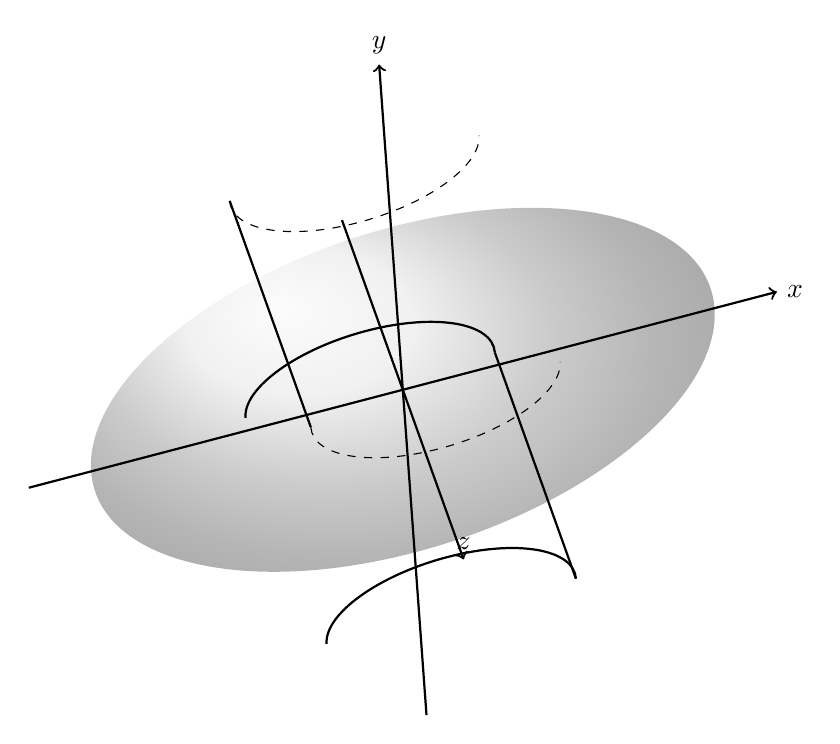
\begin{tikzpicture}
    
            % Définition de la perspective
            \begin{scope}[scale=1.5, rotate around x=10, rotate around y=30]
        
                % Boule irrégulière (ellipsoïde en 3D)
                \shade[ball color=gray!30, opacity=0.5] (0,0,0) ellipse (2.5 and 1.5);
        
                % Cylindre : bases et côtés
                \draw[thick] (1,-1,-2) -- (1,-1,2);
                \draw[thick] (-1,1,-2) -- (-1,1,2);
                
                % Dessin des bases du cylindre
                \draw[thick] (1,-1,2) arc[start angle=0, end angle=180, x radius=1, y radius=0.5];
                \draw[dashed] (-1,1,2) arc[start angle=180, end angle=360, x radius=1, y radius=0.5];
                
                \draw[thick] (1,-1,-2) arc[start angle=0, end angle=180, x radius=1, y radius=0.5];
                \draw[dashed] (-1,1,-2) arc[start angle=180, end angle=360, x radius=1, y radius=0.5];
        
                % Axes orthonormés
                \draw[thick,->] (-3,0,0) -- (3,0,0) node[right] {$x$};
                \draw[thick,->] (0,-3,0) -- (0,3,0) node[above] {$y$};
                \draw[thick,->] (0,0,-3) -- (0,0,3) node[above] {$z$};
        
            \end{scope}
        
        \end{tikzpicture}
    \end{center}
\end{comment}

\begin{definition}[Fonction Lipschitzienne en la variable d'état]
    Soit 
    \[ f : 
        \begin{cases}
            \Omega = I \times \Omega' \longrightarrow \K^n \\ 
            (t,x) \longmapsto f(t,x)
        \end{cases} \] 
    On dit que $f$ est LVE (lipschitzienne en la variable d'état i.e $x$) \underline{si} :
    \[ \forall J \in I \text{ compact } \exists k \in \R_+ \text{ tel que } : \] 
    \[ \forall t \in J, \forall x, x' \in \Omega', \quad \boxed{\| f(t,x) - f(t,x')\| \leqslant k \| x - x' \| } \]  
\end{definition}

\begin{remark}
    Une fonction lipschitzienne en la variable d'état est localement lipschitzienne en la variable d'état. 
    \[ \text{i.e} \quad LVE \Longrightarrow LLVE \] 
\end{remark}

\begin{example}
    Soit $f : (t,x) \longmapsto A(t)x + B(t)$. Supposons que $A, B \in \mathcal{C}^0(I, \mathcal{M}_n(\K))$.

    $f$ est LVE car $ \forall t \in J, x,x' \in \K^n$ où $J \subset I$, on a : 
        \begin{align*}
            \| f(t,x) - f(t,x') \| &= \| A(t) (x-x') \| \\ 
            & \leqslant \| A(t)\| \times \| x-x'\| \\ 
            & \leqslant \sup_{t \in J} \| A(t) \| \in \R_+ 
        \end{align*}
\end{example}

\begin{theorem}[Cauchy-Lipschitz LVE]
    Soit 
        \[ (P) : 
            \begin{cases}
                (E) : y'(t) = f(t,y) \\ 
                (C) : y(t_0) = y_0
            \end{cases} 
        \quad \text{où } f : I \times \Omega \overset{\text{LVE}}{\longrightarrow} \K^n \] 
    \underline{Alors} il existe une unique solution maximale au problème de Cauchy $(P)$. 
    Cette solution est même globale. 
\end{theorem}

\begin{theorem}[Cauchy-Lipschitz LLVE]
    Soit 
        \[ (P) : 
            \begin{cases}
                (E) : y'(t) = f(t,y) \\ 
                (C) : y(t_0) = y_0
            \end{cases} 
        \quad \text{où } f : I \times \Omega \overset{\text{LLVE}}{\longrightarrow} \K^n \] 
    \underline{Alors} il existe une unique solution \textbf{maximale} au problème de Cauchy $(P)$. 
\end{theorem}

\textbf{Attention : } Cette solution n'est pas forcément globale. 

\begin{example}
    \[ f : 
        \begin{cases}
            \R \times \R \longrightarrow \R \\ 
            (t,x) \longmapsto x^2
        \end{cases} 
        \quad \text{LLVE mais non LVE} 
        \quad  g : 
        \begin{cases}
            R \times R \longrightarrow \R \\ 
            (t,x) \longmapsto \sqrt{|x|}
        \end{cases}
        \quad \mathcal{C}^0 \text{ mais pas LLVE} \] 
\end{example}

En pratique nous utiliserons plutôt le résultat suivant pour invoquer le théorème de Cauchy-Lipschitz. 

\begin{proposition}
    Toute fonction $ \mathcal{C}^1$ par rapport à la variable d'état est LLVE. 
\end{proposition}


\subsection{Équations à variables séparables}

\begin{definition}[Équation différentielle à variable séparable]
    Une équation différentielle à variables séparables est une équation différentielle scalaire de la forme : 
        \[ (E) : y'(t) = f(y)g(t) \] 
    où : 
    \begin{itemize}
        \item $f : \Omega \overset{ \mathcal{C}^0}{\longrightarrow} \K $
        \item $g : I \overset{ \mathcal{C}^0}{\longrightarrow} \K $ 
    \end{itemize}
\end{definition}

\begin{example}
    Quelques exemples d'équation différentielles à variables séparables : 

\end{example}

\subsection{Théorème de sortie de tout compact}

\begin{theorem}[Sortie de tout compact]
    Soit $(E) : y'(t) = f(t,y)$ sur $]a,b[$ où : 
        \[ f : ]a,b[ \times \Omega \longrightarrow \K^n \] 
    Soit $y : ]c,d[ \longrightarrow \K^n$ une solution maximale de $(E)$ non globale telle que $d < b$. 

    \underline{Alors} $ \forall K \subseteq \Omega$ compact, il existe un voisinnage $V$ de $d$ tel que : 
        \[ \forall t \in V, y(t) \not \in K \] 
\end{theorem}

\begin{comment}
    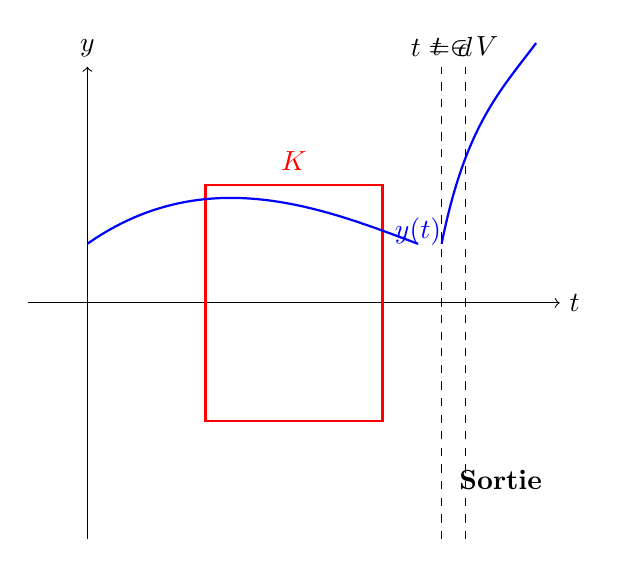
\begin{tikzpicture}[scale=1.5]
        % Axes
        \draw[->] (-0.5,0) -- (4,0) node[right] {$t$};
        \draw[->] (0,-2) -- (0,2) node[above] {$y$};
        
        % Domaine d'existence
        \draw[dashed] (3,-2) -- (3,2) node[above] {$t=d$};
        
        % Compact K
        \draw[thick, red] (1, -1) rectangle (2.5, 1);
        \node[red] at (1.75,1.2) {$K$};
        
        % Solution y(t)
        \draw[thick, blue] (0,0.5) .. controls (1,1.2) and (2,0.8) .. (2.8,0.5);
        \node[blue] at (2.8,0.6) {$y(t)$};
        
        % Zone après d
        \draw[dashed] (3.2,-2) -- (3.2,2) node[above] {$t \in V$};
        
        % Sortie du compact
        \draw[thick, blue] (3,0.5) .. controls (3.2,1.5) and (3.5,1.8) .. (3.8,2.2);
        \node at (3.5,-1.5) {\textbf{Sortie}};
    \end{tikzpicture}
\end{comment}

\begin{theorem}[Explosion]
    Avec les mêmes hypothèses et $\Omega = \K^n$, on a : 
    \begin{itemize}
        \item Si $b > d$ alors $ \| y(t) \| \underset{t \to d}{\longrightarrow} \infty $ 
            \begin{quote}
                Par contraposée, si $ \| y(t) \| \underset{t \to d}{ \not \longrightarrow} \infty $ 
                (i.e $y$ est bornée au voisinnage de $d$) alors $b = d$
            \end{quote}
        \item Si $y$ est bornée alors elle est globale. 
        \item Si $f$ est bornée alors toute fonction maximale est globale. 
    \end{itemize}
\end{theorem}


\subsection{Flot d'une équation différentielle}

\begin{definition}[Flot]
    Soit $(E) : y'(t) = f(t,y)$ où 
        \[ f : \Omega \subset \R \times \K^n \longrightarrow \K^n \quad \text{LLVE} \] 
    Le flot de cette équation est la fonction : 
        \[ \Phi : 
            \begin{cases}
                D \longrightarrow \K^n \\ 
                (t,t_0, y_0) \longmapsto y_{t_0, y_0}(t) 
            \end{cases} \] 
    où 
    \begin{itemize}
        \item $y_{t_0, y_0}$ est l'unique solution maximale de $(E)$ qui vérifie $y(t_0) = y_0$. 
        \item $D = \{(t,t_0, y_0) \; | \; t \in I_{t_0, y_0}\} $
        \item $I_{t_0, y_0}$ est le domaine de définition de $t_0$ et $y_0$
    \end{itemize}
\end{definition}

\begin{prop}[Flot]
    \begin{itemize}
        \item $D$ est un ouvert 
        \item $\Phi$ est localement lipschitzienne (et donc $ \mathcal{C}^0$)
        \item Si $f$ est $ \mathcal{C}^p$ alors $\Phi$ est $ \mathcal{C}^p$. 
    \end{itemize}
\end{prop}

\begin{definition}[Equation Différentielle à paramètre]
    Une équation différentielle à paramètre est une famille d'équation différentielles 
        \[ (E_\lambda) \; \text{où} \; E_\lambda : y'(t) = f(t,y) \] 
        \[ \text{et } \;  f : 
            \begin{cases}
                \Omega \times \Lambda \longrightarrow \K^n \\ 
                (t,x,\lambda) \longmapsto f(t,x,\lambda)
            \end{cases} \] 
\end{definition}

\begin{definition}[Flot d'une équation différentielle à paramètre]
    Soit $(E_\lambda)$ une famille d'équation différentielles à parmaètre telle que $ \forall \lambda \in \Lambda$ 
    on ait :
        \[ f(.,.,\lambda) \; \text{LLVE} \] 
    Le flot paramétré est : 
        \[ \Phi : 
            \begin{cases}
                D \longrightarrow \K^n \\ 
                (t,t_0,y_0,\lambda) \longmapsto y_{t_0, y_0, \lambda}(t) 
            \end{cases} \] 
    où $y_{t_0, y_0, \lambda}$ est l'unique solution maximale de $(E_\lambda)$ telle que $y(t_0) = y_0$. 
\end{definition}

\begin{prop}[Flot]
    \begin{itemize}
        \item $D$ est un ouvert 
        \item $\Phi$ est localement lipschitzienne (et donc $ \mathcal{C}^0$)
        \item Si $f$ est $ \mathcal{C}^p$ alors $\Phi$ est $ \mathcal{C}^p$. 
    \end{itemize}
\end{prop}


% ==================================================================================================================================
% Introduction à l'étude Qualitative

\section{Introduction à l'étude qualitative}

En pratique, on ne peut que très rarement résoudre formellement une équation différentielle. 
On va donc cherche, à partir de la fonction qui la définit, de déduire des propriétés sur les solutions. 

\subsection{Équations Autonomes}

\begin{definition}[Équation Autonome]
    Une équation différentielle est dite autonomme si elle est de la forme : 
        \[ (A) : y'(t) = f(y(t)) \] 
    Autrement dit si la variable temporelle (i.e $t$) n'apparaît pas dans $f$. 
\end{definition}

On peut interpréter une équation autonome en physique comme une équation à la contrainte de temps n'apparaît pas. 

Posons maintenant quelques définitions supplémentaires... 

\begin{definition}[Champ de vecteurs]
    Un champ de vecteurs est une fonction continue $f : \Omega \subset \R^n \longrightarrow \R^n$ où $\Omega$ est un ouvert. 
    Intuitivement, elle associe à chaque point de l'espace $\Omega$ un vecteur. 
\end{definition}

\begin{definition}[Courbe Intégrale]
    Une courbe intégrale d'un champ de vecteur $f : \Omega \longrightarrow \R^n$ est une \textbf{courbe paramétrée} 
    $y : I \subset \R \longrightarrow \Omega$ telle que $y$ est solution maximale de l'équation autonome :
        \[ (E) : y'(t) = f(y(t)) \quad \forall i \in I \] 
\end{definition}

\begin{definition}[Trajectoire]
    Une trajectoire de $f : \Omega \longrightarrow \R^n$ est l'image d'une courbe intégrale de $f$. 
\end{definition}

\begin{definition}[Point Stationnaire]
    On dit que $ x_0 \in \Omega$ est un point stationnaire ou point d'quilibre si $f(x_0) = 0$. 
    Un point stationnaire est un point où le champ de vecteur est nul. 
\end{definition}

Ainsi, un champ de vecteur va permettre de modéliser un système en mouvement tel que l'écoulement d'un fluide. 
Une trajectoire de ce champ de vecteur sera donc la trajectoire d'une particule dans le fluide. 

\begin{proposition}
    Soit $y$ une courbe intégrale d'une équation autonome $(A)$ alors si $c \in \R$ alors la courbe :
        \[ y_c : 
            \begin{cases}
                I + c \longrightarrow \R^n \\ 
                t \longmapsto y(t - c)
            \end{cases} \] 
    est une courbe intégrale (i.e solution maximale de $A$). Elle a la même trajectoire que $y$ à translation près. 
\end{proposition}

\begin{proposition}
    Soit $(A)$ une équation autonome définie par une fonction $f$. Supposons que $f$ est localement lispchitzienne. 
    Soient :
        \begin{align*}
            y_1 : I_1 \longrightarrow \R^n \\ 
            y_2 : I_2 \longrightarrow \R^n 
        \end{align*}
    deux solutions maximales de $(A)$ telles que 
        \[ \exists t_1, t_2 \in I_1, I_2, \quad y_1(t_1) = y_2(t_2) \] 
    \underline{alors} $y_1$ et $y_2$ sont égales à translation près. 
\end{proposition}

\begin{definition}[Orbite]
    Toutes les courbes intégrales $y$ d'une équation autonome $f$ vérifiant le même problème de Cauchy ont la même trajectoire. 
    Cette trajectoire est appelée \textbf{orbite}. 
    On appelle \textbf{portrait de phase} la partition de $\Omega$ en orbites.  
\end{definition}

\begin{prop}[Orbites]
    Deux orbites sont soient disjointes soient égales. 
\end{prop}

\begin{proposition}
    Soit $y$ une courbe intégrale d'une équation autonome $(A)$. On a : 
    \begin{itemize}
        \item Si $y$ admet une limite $l$ à l'infini, alors $l$ est un point stationnaire de. 
        \item Si $y$ n'est pas injective alors $y$ est globale et périodique. 
    \end{itemize}
\end{proposition}


\subsection{Intégrales Premières et Systèmes Hamiltoniens}

\subsubsection{Intégrales Premières et Courbes de Niveau}

\begin{definition}[Intégrale Première]
    Soit $(E) : y' = f(y)$ une équation autonome où $f : \Omega \overset{\text{L.L}}{\longrightarrow} \R^n$. 
    Une fonction $E : \Omega \overset{ \mathcal{C}^1}{\longrightarrow} \R$ telle que pour toute 
    solution $y$ de $(A)$, on ait $E \circ y = c \in \R $ 
    \begin{align*}
        \text{i.e } & \text{ pour toute courbe intégrale } (y,I), \forall t \in I, \quad \frac{\partial}{\partial t} E \circ y = 0 \\ 
        \text{i.e } & \quad \langle \nabla E, f \rangle = 0 \\ 
        \text{i.e } & E \text{ est constante le long des orbites}
    \end{align*}
    est appelée \textbf{intégrale première} de $(A)$. 
\end{definition}

En physique, les intégrales premières représentent les quantités invariances de systèmes dynnamiques représentés par des équations 
autonomes. Par exemple, dans un système fermé, un intégrale première peut représenter l'énergie du système.

\begin{proposition}[Lien équation autonome/système dynnamique]
    Dans la suite du chapitre, nous prendrons l'habitude d'écrire les équation autonomes sous forme de systèmes 
    dynnamiques (système d'équation différentielles). 
    Détaillons comment passer de l'un à l'autre dans la cas quelconque. 
    
    Soit $(A) : y' = f(y)$ une équation autonome où $f : \Omega \subseteq \R^n \longrightarrow \R^n$ et 
    $y = (y_1, \dots, y_n)$. Le système dynnamique associé est simplement l'équation différentielle noté : 
        \[ \frac{\partial}{\partial t} 
        \begin{pmatrix}
            y_1(t) \\ 
            \vdots \\ 
            y_n(t)
        \end{pmatrix}
        = 
        \begin{pmatrix}
            f_1(y_1(t), \dots, y_n(t)) \\ 
            \vdots \\ 
            f_n(y_1(t), \dots, y_n(t)) 
        \end{pmatrix} \] 
    Que l'on écrit plus généralement avec une lettre différente pour chaque composante de $y$. 
\end{proposition}

\begin{definition}[Courbe de Niveau]
    Soit $(A) : y' = f(y)$ une équation autonome où $f : \Omega \longrightarrow \R^n$. 
    Soit $E : \R^n \longrightarrow \R$ une intégrale première de $(A)$. 
    Les courbes de niveaux de $E$ sont les ensembles de points $y \in \R^n $ tels que 
        \[ E(y) = c \in \R \] 
\end{definition}

\begin{example}[Oscillateur Harmonique]
    Soit l'équation différentielle autonome suivante : 
        \[ (A) : 
            \begin{cases}
                x'(t) = v(t) \\
                v'(t) = - \omega ^2 x(t)
            \end{cases}
            \quad \forall (t,\omega) \in \R \times \R \] 
    ici, $x$ représente la position d'un oscillateur et $v$ sa vitesse. 
    Une intégrale première de ce système est de la forme : 
        \[ E : 
            \begin{cases}
                R \times \R \overset{ \mathcal{C}^1}{\longrightarrow} \R \\ 
                (x,y) \longmapsto E(x,y) 
            \end{cases} \] 
    Multiplions $(A)$ par $v$. On a alors $ \forall t \in \R$ : 
        \begin{align*}
            v(t) v'(t) &= - \omega ^2 x(t)v(t) \\ 
            &= - \omega ^2 x(t)x'(t) \\ 
            \iff & v(t) v'(t) + \omega ^2 x(t) x'(t) = 0 
        \end{align*}
    Supposons que $E$ soit de la forme : $ \forall t \in \R, E : (x(t), v(t)) \longmapsto E(x(t), v(t))$.
    D'après la règle de la chaîne, on a $ \forall t \in \R$ : 
        \begin{align*}
            \frac{\partial}{\partial t} E(x(t), v(t)) &= \frac{\partial x(t)}{\partial t} \frac{\partial E}{\partial x} + \frac{\partial v(t)}{\partial t} \frac{\partial E}{\partial y}
            = x'(t) \frac{\partial E}{\partial x} + v'(t) \frac{\partial E}{\partial y}  \\
            \Longrightarrow & \frac{\partial E}{\partial x} = \omega ^2 x(t) \quad \text{et} \quad \frac{\partial E}{\partial y} = v(t) 
        \end{align*}
        On peut donc en conclure que : 
            \[ \forall t \in \R, \quad E(x(t), v(t)) = \frac{1}{2} \omega^2 x^2(t) + \frac{1}{2} v^2(t) \]  
    Réciproquement, par construction, $ \frac{\partial E}{\partial t} = 0 $. 
    Traçons maintenant quelques courbes de niveau : 
    
    \begin{center}
        \begin{minipage}{0.35\textwidth}
            \centering
            \includegraphics[scale=0.1]{./images/courbes_niveaux.png}
        \end{minipage}
        \hfill 
        \begin{minipage}{0.55\textwidth}
            Ces courbes permettent de représenter l'évolution du mouvement de l'oscillateur dans le plan. 
            Ici, plus l'énergie $C$ est élevée, plus le rayon des cercles en grand, 
            ce qui correspond à une plus grande amplitude. 

            On peut aussi les voir comme l'ensemble des orbites pour lesquelles l'énergie est égale à $C$. 
        \end{minipage}
    \end{center}
\end{example}

\begin{prop}[Orbites et Ensemble de Niveau]
    Toute orbite est incluse dans un ensemble de niveau. 
\end{prop}

Ainsi, les intégrales premières d'équations autonomes $(A)$ permettent de donner une idée de la forme des orbites formés
par les solutions de $(A)$. 

\subsubsection{Systèmes Hamiltoniens}

Il existe un cas particulier des équations autonomes appelés systèmes hamiltoniens. Ils offrent une approche plus 
simple pour l'étude des systèmes dynnamiques conservatifs, où certaines quantités sont conservées au cours du temps. 

\begin{definition}[Système Hamiltonien]
    Un système hamiltonien est une équation différentielle autonome (ou système d'équations différentielles autonomes associé) 
    pouvant être représentée par un fonction appelée \textbf{hamiltonien}. 
    Plus formellement, soit $(A) : y' = f(y)$ une équation autonome telle que $f : \Omega \longrightarrow \R^{2n}$. 
    On dit que $(A)$ est un système hamiltonien s'il existe une fonction : 
    \[ H : 
        \begin{cases}
            \Omega \overset{ \mathcal{C}^2}{\longrightarrow} \R \\ 
            (q,p) \longmapsto H(q,p) 
        \end{cases} 
        \quad \text{où } q,p \in \R^n \] 
    telle que $ \forall (q,p) \in \Omega$ on ait : 
        \[ \boxed{f(q,p) = \left( \frac{\partial H}{\partial p}, - \frac{\partial H}{\partial q} \right)  } \] 
    Cela revient donc à dire que $(A)$ peut s'écrire de la forme suivante : 
        \[ (A) : 
            \begin{cases}
                p'(t) = - \partial_q H(q,p) \\ 
                q'(t) = \partial_p H(q,p) 
            \end{cases} \] 
\end{definition}

\begin{remark}
    Tout système de dimension impaire n'est donc pas hamiltonien. 
\end{remark}

\begin{example}[Oscillateur Harmonique]
    Prenons comme exemple le cas classique d'un oscillateur harmonique gouverné par l'équation 
    différentielle : 
        \[ (A) : m x'' + kx = 0 \] 
    où : 
    \begin{itemize}
        \item $m$ est la masse de l'oscillateur 
        \item $k$ est la constante de raideur du ressort 
        \item $x(t)$ est la position de l'oscillateur à l'instant $t$. 
    \end{itemize}
    Représentons cette équation autonome sous la forme d'un système hamiltonien. 
    Posons $Y(t) = (x(t), y(t))$ on a alors $Y'(t) = (x'(t), y'(t))$. Soit la fonction suivante : 
    \[ f : 
        \begin{cases}
            \R^2 \longrightarrow \R^2 \\ 
            (x,y) \longmapsto (y, - \frac{k}{m}x)
        \end{cases} \] 
    Cela nous donne que : 
        \begin{align*}
            (A) \iff & Y'(t) = f(Y(t)) \\ 
            \iff & 
                \begin{cases}
                    x'(t) = y(t) \\ 
                    y'(t) = - \frac{k}{m} x 
                \end{cases} 
            \iff  
                \begin{cases}
                    x'(t) = \frac{1}{m} p(t) \\ 
                    p'(t) = -kx(t) 
                \end{cases}
        \end{align*}
        où $ p(t) = m x'(t)$ 
    
    Maintenant, posons : 
        \[ H : 
            \begin{cases}
                \R^2 \longrightarrow \R \\ 
                (x,p) \longmapsto \frac{p^2}{2m} + \frac{1}{2} k x^2 
            \end{cases} \] 
    $H$ est $ \mathcal{C}^\infty$ par composantes donc calculons ses dérivées partielles : 
        \[ \frac{\partial H}{\partial p} = \frac{p}{m} = x'(t) \quad \frac{\partial H}{\partial x} = k x(t) = - p'(t) \] 
    Donc $(A)$ est bien un système hamiltonien. 
\end{example}

\begin{prop}[Hamiltonien et intégrale première]
    Tout hamiltonien est une intégrale première. Autrement dit, un hamiltonien est un cas particulier d'intégrale première. 
\end{prop}

\begin{proposition}[Condition Nécessaire]
    Soit $(A) = y' = f(y)$ un système hamiltonien, alors $ \div f = 0 $. 
    En dimension 2, on a équivalence. 
\end{proposition}
